\documentclass[a4paper]{article}
\usepackage[utf8]{inputenc}
\usepackage{fullpage}
\usepackage{enumitem}
\usepackage{todonotes}
\usepackage{graphicx}
\usepackage{array}
\usepackage{mdwlist}
\usepackage{floatrow}
\usepackage{hyperref}
\usepackage{listings}
\usepackage{color}
\usepackage{multirow}
\usepackage{algorithm}
\usepackage{algorithmic}

\usepackage{tikz}
\usetikzlibrary{shapes,arrows}

\graphicspath{ {img/} }

% Set caption position
\floatsetup[figure]{capposition=bottom}

\title{{\Huge myTaxiService} \\ Project Plan Document}
\author{Jacopo Strada \and Luca Riva}
\date{February 2, 2016}

\begin{document}

\maketitle
\vfill
\begin{flushright}
Version 1.0
\end{flushright}

\newpage

\tableofcontents

\vfill

\listoffigures

\vfill

\listoftables

\vfill


% New page before new section
\let\stdsection\section
\renewcommand\section{\newpage\stdsection}

\setlength{\parindent}{0em}
\setlength{\parskip}{1em}

\section{Introduction}

\subsection{Purpose}
The purpose of this document is to take into account all the aspects of \emph{myTaxiService} project and try to make some estimations in order to predict the project dimension and how much work is needed to create the final product. This is very important in order to provide the people who have to sell the product with all the information about price and time, parameters always taken into account by the customer.

\subsection{Scope} 
In order to achieve what described before in this document we will use Function Point and COCOMO estimations in order to identify the size of the project and its cost.
Then also a planning is made, in which time divisions and resources allocations show the consistency of the estimations made before.
At the and a risk analysis in performed to consider all the possible problems that can compromise the project and how to eventually face them.

\subsection{Glossary}

\subsubsection{Definitions}

\begin{description}
\item[Client / Passenger / User :] Is a person who signed up for this service and their interest is to call a taxi or reserve  a ride.
\item[Taxi Driver :] Is a person who drives a taxi and would like to be called or reserved for a ride through this service.
\end{description}

\subsubsection{Acronyms}

\begin{description}
\item[GPS:] Global Positioning System
\item[DD:] Design Document
\item[RASD: ] Requirements and Specification Document
\item[COCOMO: ] Constructive Cost Model
\item[USC CSSE:] University of Southern California - Center for Systems and Software
Engineering
\item[ILF:] Internal Logical File
\item[EIF:] External Interface File
\end{description}

\subsection{Reference Documents}
\begin{itemize}
\item \emph{myTaxiDriver} Specification Document
\item \emph{myTaxiDriver} Requirements and Specification Document
\item \emph{myTaxiDriver} Integration Tests Document
\end{itemize}

\section{Project Size and Cost Estimation}
In order approximate size and cost of the project it was decided to employ the function points method and the COCOMO estimation. The function points are calculated by considering five different function types and their weight, which depends on the difficulty of the function itself. The result obtained with such method is at the base of the COCOMO estimation, in fact the function points are the sizing method used, with the other parameters shown in \autoref{fig:COCOMO-Settings}, to elaborate the final result.

\subsection{Function Points}

In the table below we are presenting how we have calculated function points for \emph{myTaxiService} application.

\begin{figure}[H]
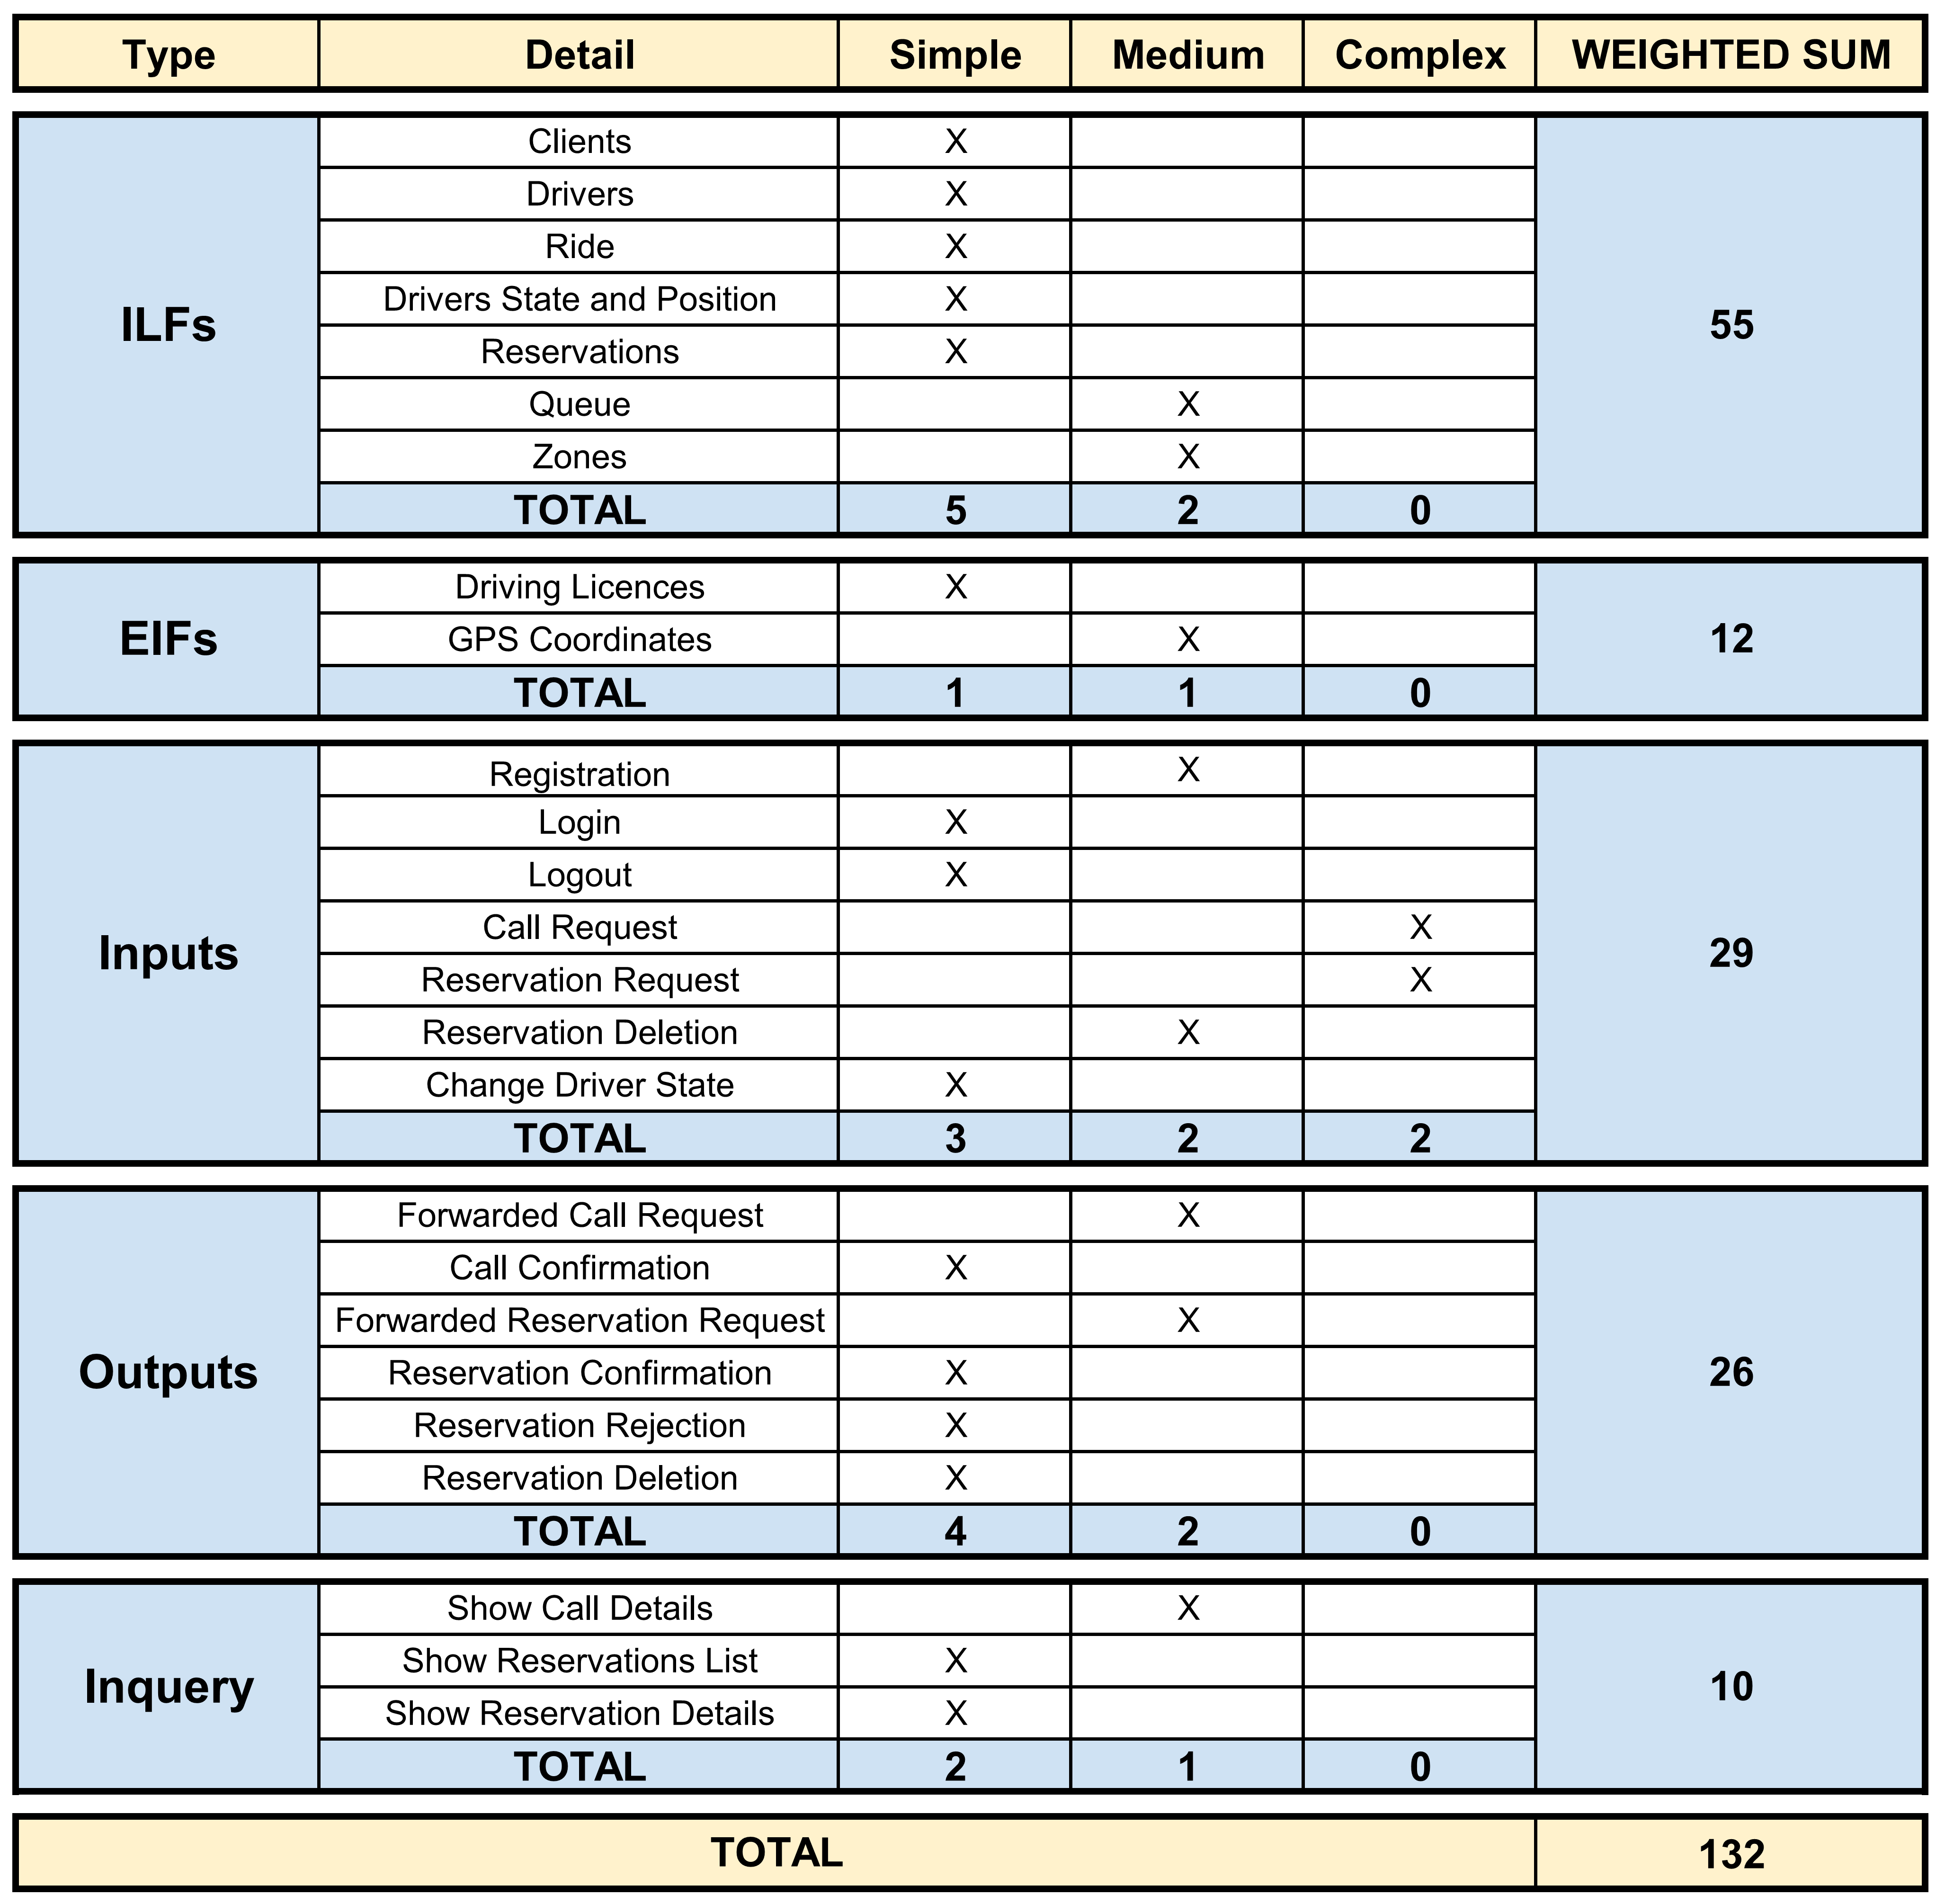
\includegraphics[width=.9\textwidth]{FunctionPoints}
\centering
\caption{Function Points}
\label{fig:FunctionPoints}
\end{figure}

\subsection{COCOMO Estimation}

In order to make the COCOMO II estimation we've used the tool given by USC CSSE. In the following figures you can see settings and results.

\begin{figure}[H]
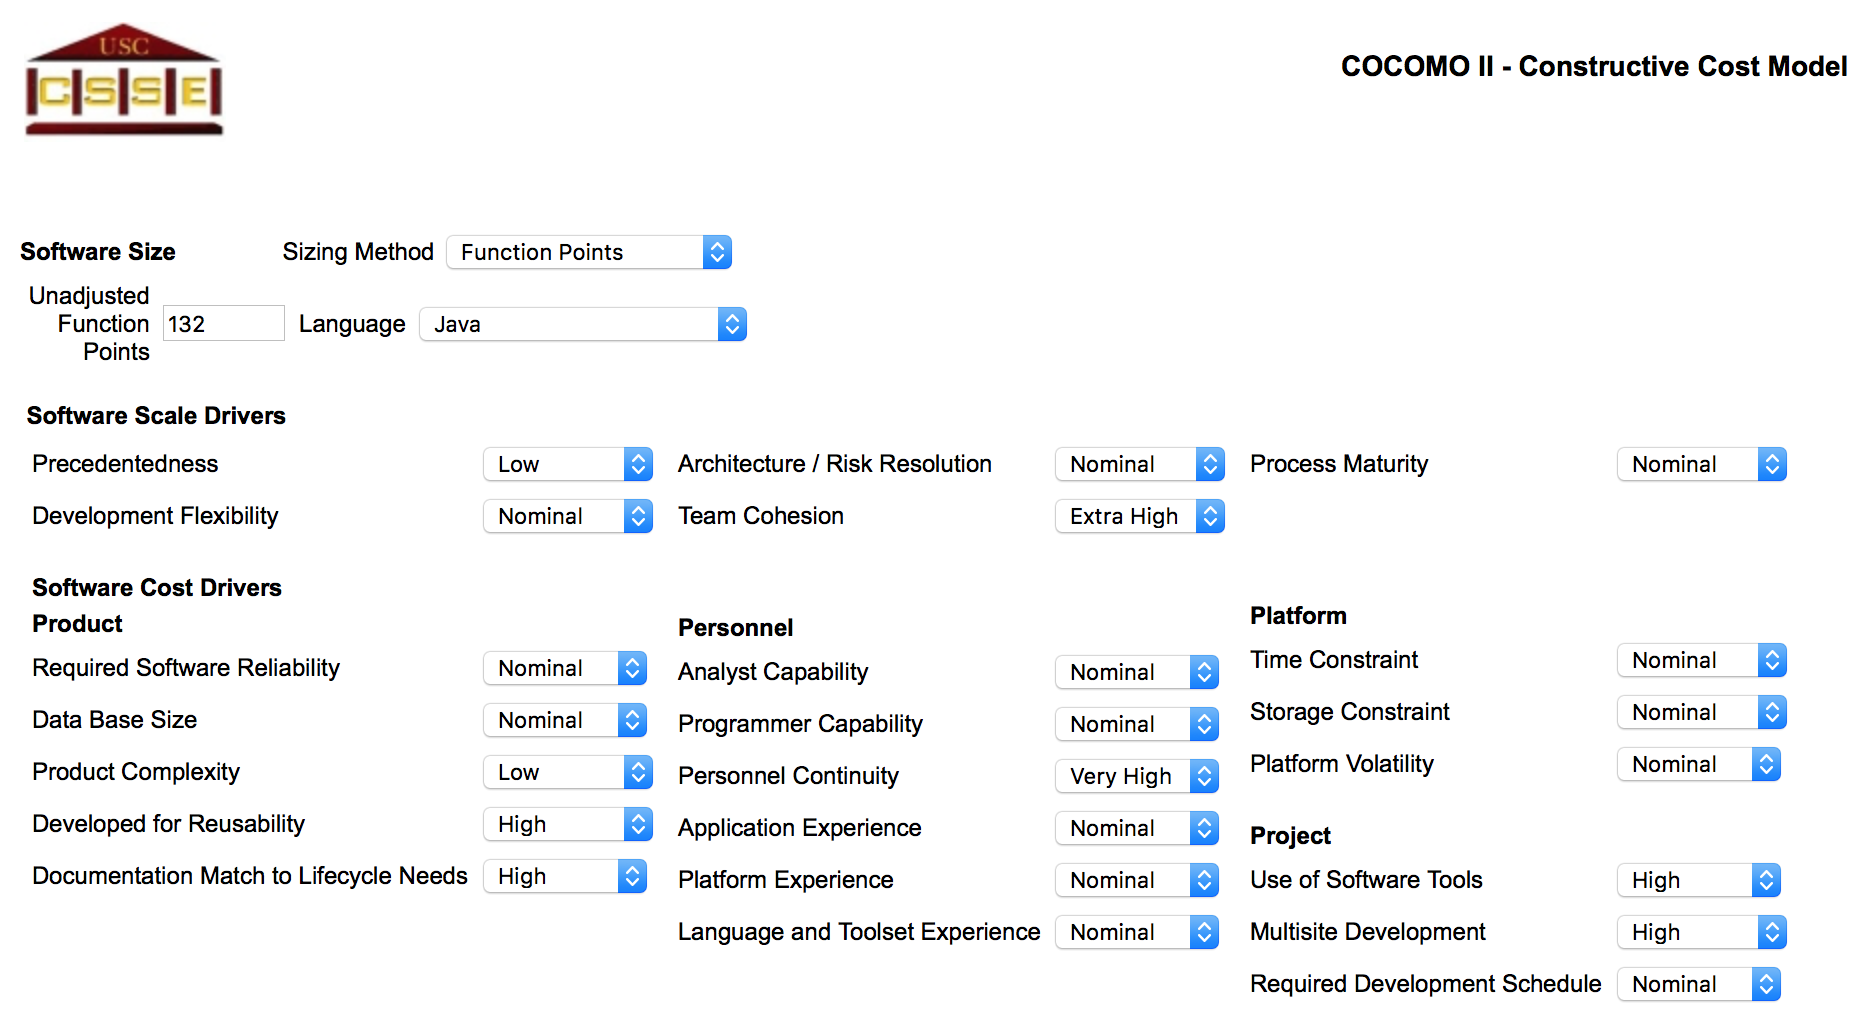
\includegraphics[width=.9\textwidth]{COCOMO-Settings}
\centering
\caption{COCOMO Settings}
\label{fig:COCOMO-Settings}
\end{figure}

\begin{figure}[H]
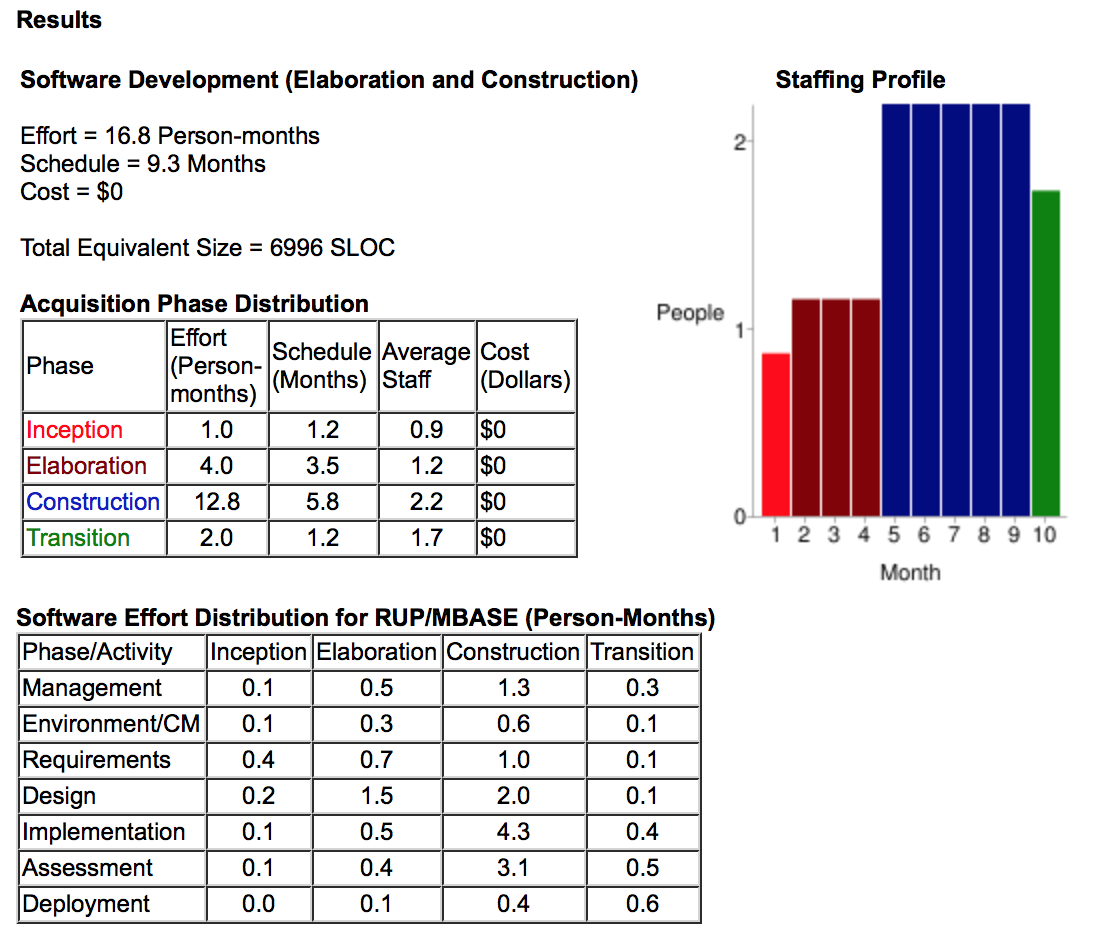
\includegraphics[width=.8\textwidth]{COCOMO-Results}
\centering
\caption{COCOMO Results}
\label{fig:COCOMO-Results}
\end{figure}

\section{Tasks, Schedule and Resource Allocation}

Having to plan all the work around \emph{myTaxiService}, first of all we have defined all the tasks to perform in order to arrive at the and of the project with a complete and functioning system.

In the following tables you can see all these tasks also grouped by type. A time for each task is also proposed and the resources have been allocated.

\vfill

\begin{figure}[H]
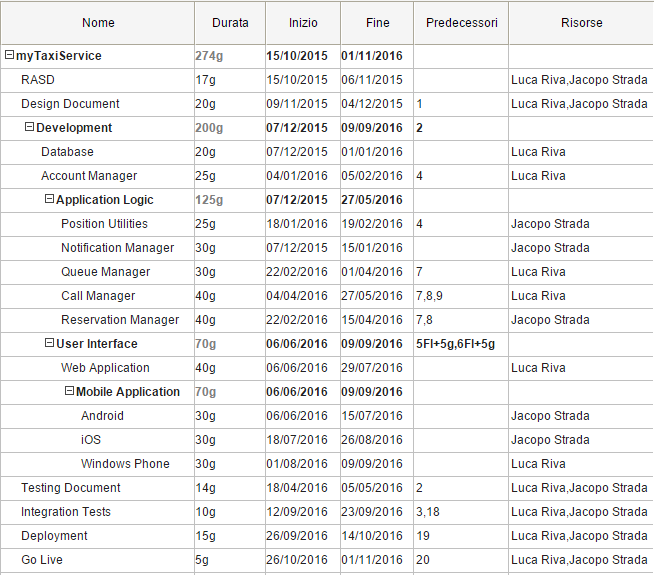
\includegraphics[width=.8\textwidth]{GANTT_TABLE}
\centering
\caption{Tasks}
\label{fig:GANTT_TABLE}
\end{figure}

\vfill

\newpage

These Gantt chart is reported in order to give a clear idea of how the team is planning to work on the various project's tasks, giving information about the expected necessary time to complete each of them. The length of the considered period was previously calculated with the COCOMO approach.

\vfill

\begin{figure}[H]
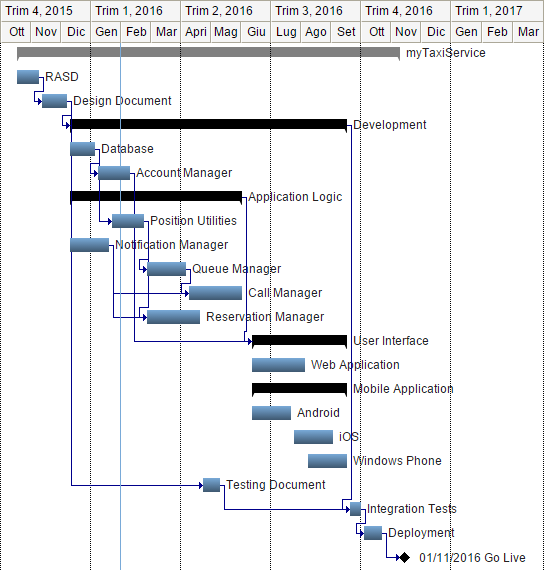
\includegraphics[width=.8\textwidth]{GANTT_CHART}
\centering
\caption{Gantt Chart}
\label{fig:GANTT_CHART}
\end{figure}

\vfill

\newpage

The last two following charts describe the tasks that each member of the team has to perform and how much time they have to perform it.

\begin{figure}[H]
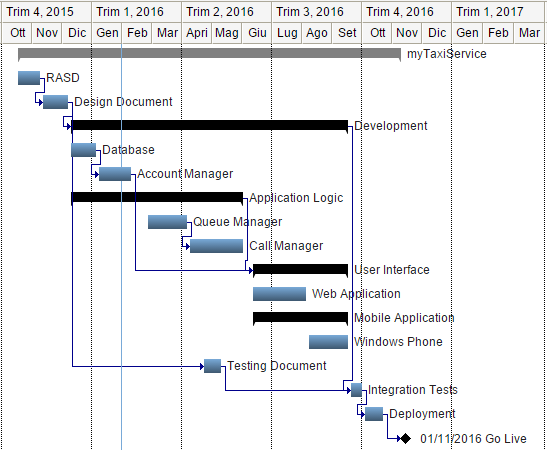
\includegraphics[width=.7\textwidth]{GANTT_CHART_LUCA}
\centering
\caption{Luca's Tasks}
\label{fig:GANTT_CHART_LUCA}
\end{figure}

\begin{figure}[H]
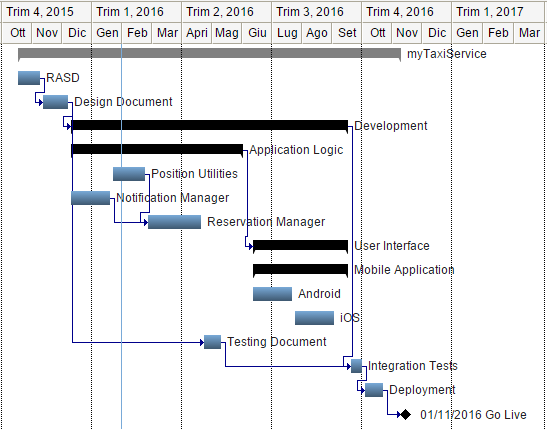
\includegraphics[width=.7\textwidth]{GANTT_CHART_JACOPO}
\centering
\caption{Jacopo's Tasks}
\label{fig:GANTT_CHART_JACOPO}
\end{figure}

\section{Project Risk}
This table reports the possible risks that may compromise the project and how we are prepared to prevent or eventually face them.
\renewcommand{\arraystretch}{2}
\newcolumntype{M}{>{\centering\arraybackslash} m }

\begin{table} [H]
\begin{center}
\begin{tabular}{ |M{.25\textwidth}|M{.13\textwidth}|M{.14\textwidth}|M{.36\textwidth}|  }
\hline \textbf{Risk} & \textbf{Probability} & \textbf{Effects} & \textbf{Strategy} \\ \hline
	\hline  Personnel shortfalls & moderate & serious & Predict the time necessary in order to develop the project
	as accurately as possible, also considering possible periods of illness or impossibility to work in general \\ 
	\hline Developing the wrong software functions & low & catastrophic & Elaborate a clear an precise requirement analysis 
	and present it to the clients in order to acknowledge if what was understood coincides with the requests. It is also
	important to keep in contact with the IT department of the customers to avoid taking crucial decision without consulting them\\
	\hline  Shortfalls of externally performed tasks & low & catastrophic & Always keep in mind eventual alternatives and write a software
	which is not too much attached to a specific API, so that it would be possible to change the external provider much faster. \\
	\hline Failure to gain users commitment & moderate & serious & Convince the stakeholders to invest also in advertisement both
	in the city and on the Web\\
	\hline Inadequate estimation of required resources & moderate & catastrophic & Convince the stakeholders to buy hardware with
	more performances and simplify as possible the most computational parts of the software\\
	\hline  High level of level of technical complexity & low & serious & Evaluate the possibility to address a consultant to help in the
	most critical parts of the development\\
	\hline Customer financial problems & moderate & catastrophic & Develop a project which is scalable and adaptable to other circumstances
	in order to be sold also in other markets to new clients\\
	\hline
\end{tabular}
\end{center}
\caption{Risks}
\label{table:risks}
\end{table}


\section{Appendix}

\subsection{Software and Tools used}

\begin{description}
\item[ShareLatex:] This web application was used to redact this document in a collaborative way. 
\newline (\url{https://it.sharelatex.com/})
\item[Ganterr:] This web application was used to create the Gantt chart
\newline (\url{https://www.smartapp.com/gantterforgoogledrive/})
\item[Csse COCOMOII tool] This web application was used to evaluate the COCOMO
\newline(\url{http://csse.usc.edu/tools/COCOMOII.php})
\item[Google Sheets] This web application was used to calculate Function Points
\newline(\url{http://sheets.google.com})
\end{description}

\subsection{Hours of Work}
We spent approximately the following amount of hours to redact this document:
\begin{description}
\item[Riva Luca:] 10
\item[Strada Jacopo:] 10 
\end{description}

\subsection{Gantt Chart in higher resolution}
\nopagebreak
Here is the Gantt Chart in a higher resolution in order to see better the granularity of tasks.
\nopagebreak
\begin{figure}[H]
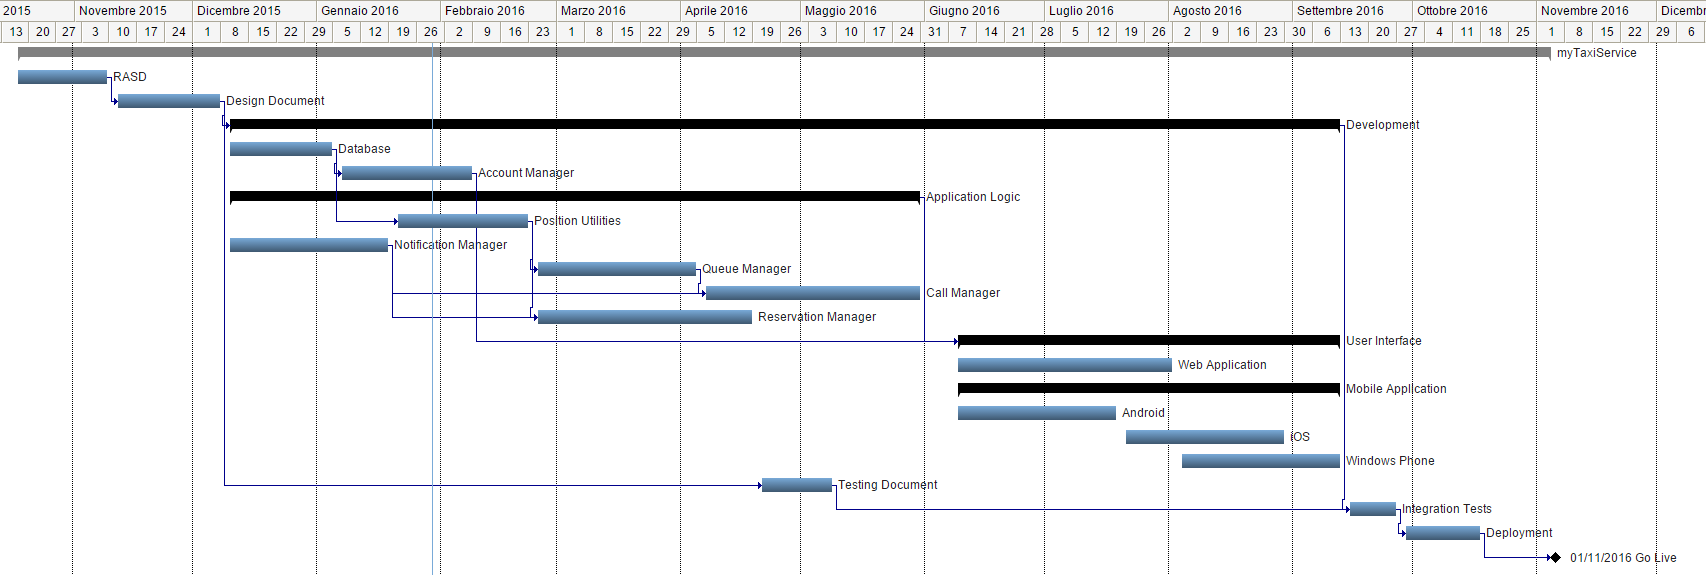
\includegraphics[width=.88\textheight, angle =90]{GANTT_CHART_BIG}
\centering
\caption{Gantt Chart in higher resolution}
\label{fig:GANTT_CHART_BIG}
\end{figure}

\end{document}